\subsection{Integers over a graded ring}

All the graduations considered in this no. are of type Z; if A is a graded ring and \(i \in Z\) , \(A_{i}\) denotes the set of homogeneous elements of degree i of the ring A.

Let A be a graded ring and B a graded A-algebra. Let x be a homogeneous element of B which is integral over A; then there is a relation

\[
x ^ {n} + a _ {1} x ^ {n - 1} + \dots + a _ {n} = 0 \quad \text { where } \quad a _ {i} \in A \quad \text { for } \quad 1 \leqslant i \leqslant n.\tag{3}
\]

Let \(m = \deg(x)\) and let \(a_i'\) be the homogeneous component of degree \(mi\) of \(a_i\) ( \(1 \leqslant i \leqslant n\) ); then obviously

\[
x ^ {n} + a _ {1} ^ {\prime} x ^ {n - 1} + \dots + a _ {n} ^ {\prime} = 0\tag{4}
\]

in other words x satisfies an equation of integral dependence with homogeneous coefficients.

Let \(\mathbf{A}[\mathbf{X},\mathbf{X}^{-1}]\) denote the ring of fractions \(\mathbf{S}^{-1}\mathbf{A}[\mathbf{X}]\) of the polynomial ring \(\mathbf{A}[\mathbf{X}]\) in one indeterminate, \(\mathbf{S}\) being the multiplicative subset of \(\mathbf{A}[\mathbf{X}]\) consisting of the powers \(\mathbf{X}^n\) of \(\mathbf{X}\) ( \(n\geqslant 0\) ); as \(\mathbf{X}\) is not a divisor of 0 in \(\mathbf{A}[\mathbf{X}]\) it is immediate that the \(\mathbf{X}^i\) ( \(i\in \mathbf{Z}\) ) form a basis over \(\mathbf{A}\) of the A-module \(\mathbf{A}[\mathbf{X},\mathbf{X}^{-1}]\) . For every element \(a\in \mathbf{A}\) with homogeneous components \(a_{i}\) ( \(i\in \mathbf{Z}\) ), we write

\iffalse
\begin{description}
\tightlist
\item[\$\$]
j \_ \{\mathbf {A}\} (a) = \sum\_ \{i \in \mathbf {Z}\} a \_ \{i\} \mathbf {X} \^{} \{i\} \in \mathrm{A} {[} \mathbf {X}, \mathbf {X} \^{} \{- 1\} {]}\tag{5} \$\$
\end{description}
\fi

\[
:j_{A}(a) = \sum_{i \in \mathbf{Z}} a_{i} \mathbf{X}^{i} \in \mathbf{A}[\mathbf{X},\mathbf{X}^{-1}]\tag{5}
\]

it is immediate that \(j_{A}: A \to A[X, X^{-1}]\) is an injective ring homomorphism.

PROPOSITION 20. Let \(\mathbf{A} = \bigoplus_{i\in \mathbf{Z}}\mathbf{A}_i\) be a graded ring and \(\mathbf{B}\) a (commutative) graded A-algebra. The set \(\mathbf{A}'\) of elements of \(\mathbf{B}\) integral over \(\mathbf{A}\) is a graded subalgebra of \(\mathbf{B}\) . If \(\mathbf{A}_i = 0\) for \(i < 0\) and \(\mathbf{B}\) is a reduced ring, then \(\mathbf{A}_i' = 0\) for \(i < 0\) .

If \(\mathbf{A}_i = 0\) for \(i < 0\) and \(\mathbf{B}\) is a reduced ring, then \(\mathbf{A}_i' = 0\) for \(i < 0\) . The diagram

\pandocbounded{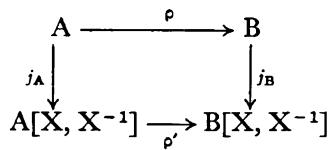
\includegraphics[keepaspectratio]{images/part002_18d5f867.jpg}}

(where \(\rho\) is the homomorphism defining the A-algebra structure on B and \(\rho'\) the homomorphism canonically derived from it) is commutative, as is immediately verified from the definition (5). Let \(x\) be an element of B integral over A; then \(j_{\mathrm{B}}(x)\) is integral over \(\mathbf{A}[\mathbf{X}, \mathbf{X}^{-1}]\) (no. 1, Proposition 2) and it therefore follows from no. 5, Proposition 16 that there exists an integer \(m > 0\) such that \(\mathbf{X}^m j_{\mathrm{B}}(x)\) is an element of \(\mathbf{B}[\mathbf{X}]\) integral over \(\mathbf{A}[\mathbf{X}]\). We then deduce from no. 3, Proposition 12 that the coefficients of the polynomial \(\mathbf{X}^m j_{\mathrm{B}}(x)\) are integral over A; as these coefficients are by definition the homogeneous components of \(x\) , it is seen that these are integral over A, which proves that \(\mathbf{A}'\) is a graded subalgebra of B.

Suppose now that \(x \in \mathbf{A}_i'\) where \(i < 0\) ; the remark at the beginning of this no. shows that \(x\) satisfies an equation of the form (4) where \(a_k' \in \mathbf{A}_{ki}\) for \(1 \leqslant k \leqslant n\) . If \(\mathbf{A}_j = 0\) for \(j < 0\) , then \(x^n = 0\) and if \(B\) is a reduced ring we conclude that \(x = 0\) and hence \(\mathbf{A}_i' = 0\) for all \(i < 0\) in this case.

Recall (Chapter II, § 2, no. 9) that, if \(\mathbf{A} = \bigoplus_{i\in \mathbf{Z}}\mathbf{A}_i\) is a graded ring and S is a multiplicative subset of A consisting of homogeneous elements, a graded ring structure is defined on \(\mathrm{S}^{-1}\mathrm{A}\) by taking the set \((\mathrm{S}^{-1}\mathrm{A})_i\) of homogeneous elements of degree \(i\) to be the set of elements of the form \(a / s\) , where \(a\in \mathbf{A}\) and \(s\in \mathbf{S}\) are homogeneous and such that \(\deg (a) - \deg (s) = i\) .

LEMMA 4. Let \(\mathbf{A} = \bigoplus_{i\in \mathbf{Z}}\mathbf{A}_i\) be a graded integral domain and S the set of homogeneous elements \(\neq 0\) of A.

\begin{enumerate}
\def\labelenumi{(\roman{enumi})}
\item
  Every homogeneous element \(\neq 0\) of \(\mathbf{S}^{-1}\mathbf{A}\) is invertible, the ring \(\mathbf{K}_0 = (\mathbf{S}^{-1}\mathbf{A})_0\) is a field and the set of \(i\in \mathbf{Z}\) such that \((\mathrm{S}^{-1}\mathrm{A})_i\neq 0\) is a subgroup \(q\mathbf{Z}\) of \(\mathbf{Z}\) (where \(q\geqslant 0\) ).
\item
  Suppose that \(q \geqslant 1\) and let \(t\) be a non-zero element of \((\mathbf{S}^{-1}\mathbf{A})_q\) . Then the \(\mathbf{K}_0\) -homomorphism \(f\) of the polynomial ring \(\mathbf{K}_0[\mathbf{X}]\) to \(\mathbf{S}^{-1}\mathbf{A}\) which maps \(\mathbf{X}\) to \(t\) extends to an isomorphism of \(\mathbf{K}_0[\mathbf{X}, \mathbf{X}^{-1}]\) onto \(\mathbf{S}^{-1}\mathbf{A}\) and \(\mathbf{S}^{-1}\mathbf{A}\) is integrally closed.
\end{enumerate}

The assertions in (i) follow immediately from the definitions and the hypothesis that A is an integral domain, for if \(a/s\) and \(a'/s'\) are two homogeneous elements \(\neq 0\) of \(\mathrm{S}^{-1}\mathrm{A}\) of degrees \(i\) and \(i'\) , \(aa'/ss'\) is a homogeneous element \(\neq 0\) and of degree \(i+i'\) . To show (ii), we note that since \(t\) is invertible in \(\mathrm{S}^{-1}\mathrm{A}\) the homomorphism \(f\) extends in a unique way to a homomorphism \(\bar{f}: \mathrm{K}_0[\mathrm{X}, \mathrm{X}^{-1}] \to \mathrm{S}^{-1}\mathrm{A}\) and necessarily \(\bar{f}(\mathrm{X}^{-1}) = t^{-1}\) . On the other hand, by definition of \(q\) , every homogeneous element \(\neq 0\) of \(\mathrm{S}^{-1}\mathrm{A}\) is of degree \(qn\) ( \(n \in \mathbf{Z}\) ) and hence can be written uniquely in the form \(\lambda t^n\) where \(\lambda \in \mathrm{K}_0\) (since \(\mathrm{S}^{-1}\mathrm{A}\) is an integral domain); hence \(\bar{f}\) is bijective. Finally, we know that \(\mathrm{K}_0[\mathrm{X}]\) is integrally closed (no. 3, Proposition 10) and hence so is \(\mathrm{K}_0[\mathrm{X}, \mathrm{X}^{-1}]\) (no. 5, Corollary 1 to Proposition 16), which completes the proof of the Lemma.

PROPOSITION 21. Let \(\mathbf{A} = \bigoplus_{i\in \mathbf{Z}}\mathbf{A}_i\) be a graded integral domain and S the set of homogeneous elements \(\neq 0\) of A. The integral closure \(\mathbf{A}'\) of A is then a graded subring of \(\mathbf{S}^{-1}\mathbf{A}\) . If further \(\mathbf{A}_i = 0\) for \(i < 0\) , then \(\mathbf{A}_i' = 0\) for \(i < 0\) .

If \(A = A_{0}\) , the proposition is trivial. Otherwise we may apply Lemma 4; the ring \(S^{-1}A\) is an integrally closed domain and therefore \(A' \subset S^{-1}A\) ; as \(S^{-1}A\) is graded, so is \(A'\) by Proposition 20; the latter assertion also follows from Proposition 20.

COROLLARY 1. With the hypotheses and notation of Proposition 21, if every homogeneous element of \(\mathbf{S}^{-1}\mathbf{A}\) which is integral over \(\mathbf{A}\) belongs to \(\mathbf{A}\) , then \(\mathbf{A}\) is integrally closed.

Then \(\mathbf{A}_i' \subset \mathbf{A}\) for all \(i \in \mathbf{Z}\) and hence \(\mathbf{A}' = \mathbf{A}\) .

COROLLARY 2. If \(\mathbf{A} = \bigoplus_{i\in \mathbf{Z}}\mathbf{A}_i\) is an integrally closed graded domain, the domain \(\mathbf{A}_0\) is integrally closed.

The field of fractions \(\mathbf{K}_0\) of \(\mathbf{A}_0\) is identified (in the notation of Proposition 21)

with a subring of the ring of homogeneous elements of degree 0 of \(S^{-1}A\) ; every element of \(K_{0}\) integral over \(A_{0}\) (and a fortiori over A) belongs therefore by hypothesis to \(A_{0}\) .

COROLLARY 3. Let \(\mathbf{A} = \bigoplus_{i\in \mathbf{Z}}\mathbf{A}_i\) be an integrally closed graded domain. Then, for every integer \(d > 0\) , the ring \(\mathbf{A}^{(d)}\) (Chapter III, §1, no. 3) is an integrally closed domain.

Let U be the set of homogeneous elements \(\neq0\) of \(A^{(d)}\) and let x be a homogeneous element of \(U^{-1}A^{(d)}\) integral over \(A^{(d)}\) and hence over A; as \(x\in S^{-1}A\) , x belongs to A by hypothesis; as its degree is divisible by d, it belongs to \(A^{(d)}\) and it then follows from Corollary 1 that \(A^{(d)}\) is integrally closed.

